\documentclass[10pt]{article}

\usepackage{spheric}
%%%TITLE
\title{Construction of Two-dimensional SPH Numerical Wave Tank}
\date{}

%%AFFILIATIONS
\author[$\relax$]{Jingyu Wang}
\author[$\relax$]{Fei Xu$^\dagger$}
\author[$\relax$]{Yang Yang}

\affil[$\relax$]{School of Aeronautics, Northwestern Polytechnical University, 710072, Xi'an, P.R.China}
\affil[$\relax$]{\email{\dagger}{xufei@nwpu.edu.cn}}

%%DOCUMENT
\begin{document}

\maketitle

%\SelectedTopics{}

%%PLEASE PUT YOUR ABSTRACT HERE
\begin{abstract}
The numerical wave tank is one of the effective tools to study the wave and its effect on the floating structure. Compared with the traditional methodology of CFD to construct the tank, the Smoothed Particle Hydrodynamics (SPH) method is superior in dealing with problems concerning complex boundary and large deformation.

In this paper, a numerical wave tank is established and verified based on the SPH method. The main contents of the paper are as follows. Firstly, the mathematical derivation of discrete calculation of Navier-Stokes control equations is completed, based on the fundamental concepts of SPH method and accompanied with relevant numerical processing techniques. The repulsive function is employed to simulate the interaction between the swinging plate and the water. Secondly, adopted the linear wave-maker theory, the calculation process of numerical simulation of swinging plate is given, in which the amplitude and circular frequency of the swinging plate can be obtained by solving the continuous equation. In the construction of the numerical tank, apart from the swinging plate at the upstream that excites the motion of water to generate the required waves, an artificial viscosity sponge layer is introduced at the downstream to remove the unwanted wave reflections from the boundaries, which ensures the wave characteristic of the workspace.

During the construction of the numerical pool, the following work is carried out: (i) The technical parameters in artificial viscosity, boundary treatment and free surface recognition in the SPH method are thoroughly investigated. (ii) Wave generation and propagation in the numerical wave tank is tested and confirmed with analytical results. (iii) The influence of swinging speed, the immersion of the swinging plate and the depth of water on the generation of various wave are discussed.

\begin{figure}[!htb]
\centering
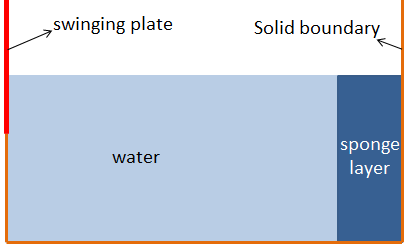
\includegraphics[width=0.4\textwidth]{28-1.png}
\caption{Model of two-dimensional wave tank}\label{fig:28-1}
\end{figure}

\begin{figure}[!htb]
\centering
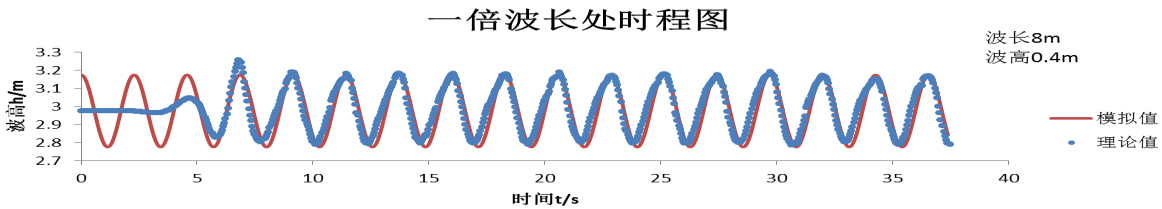
\includegraphics[width=0.9\textwidth]{28-2.png}
\caption{Results of linear regular wave generating}\label{fig:28-2}
\end{figure}

\end{abstract}


%%THE END OF ABSTRACT

\addbib

\end{document}
